\documentclass[aspectratio=169]{beamer}
\geometry{paperwidth=160mm,paperheight=100mm}
\usepackage{beamerthemesidebar}
\usepackage{hyperref}
\usepackage{color}
\usepackage{multimedia}
\usepackage{colortbl}
\usepackage{amsmath}
\usepackage{empheq}
\usepackage{cancel}
\usepackage{amssymb}
\usepackage{amsfonts}
\usepackage{lipsum}
\usepackage{tcolorbox}
\usepackage{tabularx}
\usepackage{caption}
\usepackage{bm}

\setbeamersize{sidebar width right=0pt}
\setbeamertemplate{footline}[frame number]
%
\definecolor{orange}{RGB}{250,167,12}
\definecolor{yellow}{RGB}{246,250,12}
\definecolor{green}{RGB}{128,238,1}
\definecolor{black}{RGB}{0,0,0}
\definecolor{blue}{RGB}{0,0,255}
\definecolor{red}{RGB}{255,0,0}
\definecolor{sepia}{RGB}{94,38,18}
\newcommand{\ve}[1]{{\rm\bf {#1}}}
\newcommand{\q}[1]{\textcolor{blue}{#1}}
\newcommand{\blue}[1]{\textcolor{blue}{#1}}
\newcommand{\sepia}[1]{\textcolor{sepia}{#1}}
\newcommand{\red}[1]{\textcolor{red}{#1}}
\newcommand{\green}[1]{\textcolor{green}{#1}}
\newcommand{\yellow}[1]{\textcolor{yellow}{#1}}
\newcommand{\orange}[1]{\textcolor{orange}{#1}}
\definecolor{burlywood}{RGB}{255,211,155}
\definecolor{chocolate}{RGB}{255,127,36}
\definecolor{tan}{RGB}{210,180,140}
%
\def\onethird{{\textstyle{1\over3}}}
\def\twothirds{{\textstyle{2\over3}}}
\def\fourthirds{{\textstyle{4\over3}}}
\def\onehalf{{\textstyle{1\over2}}}
\def\threehalfs{{\textstyle{3\over2}}}
%
\newcommand{\pd}{\partial}
\newcommand{\aMLT}{\alpha_{\rm MLT}}
\newcommand{\Fconv}{F_{\rm conv}}
\newcommand{\Frad}{F_{\rm rad}}
\newcommand{\Ftot}{F_{\rm tot}}
\newcommand{\Hp}{H_p}
\newcommand{\prad}{p_{\rm rad}}
\newcommand{\pgas}{p_{\rm gas}}
\newcommand{\TTc}{T_{\rm c}}
\newcommand{\rhoc}{\rho_{\rm c}}
\newcommand{\Teff}{T_{\rm eff}}
\newcommand{\Fstar}{F_\star}
\newcommand{\pstar}{p_\star}
\newcommand{\Pstar}{P_\star}
\newcommand{\Rstar}{R_\star}
\newcommand{\rhostar}{\rho_\star}
\newcommand{\Tstar}{T_\star}
%
\title{Theoretical Astrophysics I: Physics of Sun and Stars\\
Lecture 8: Detailed Models of Stellar Evolution}
\author{\texorpdfstring{\sepia{Petri K\"{a}pyl\"{a} Ivan Mili\'{c}}\newline\blue{\url{pkapyla, milic@leibniz-kis.de}}}{}}
\institute{Institut f\"ur Sonnenphysik - KIS, Freiburg}
\date{\today}
%
\begin{document}
\frame{\titlepage}


\section{Evolution of stars - detailed picture}
%
\frame{
\frametitle{Detailed picture of stellar evolution}
\begin{itemize}
\item As opposed to the simple treatment we have adopted so far, a
  general treatment of stellar evolution needs to take into account
  the details of opacity, nuclear energy production, and equation of
  state.
\item Then the equations of stellar evolution need to be solved
  \emph{numerically} and due to their non-linearity results that might
  not be intuitively clear can arise.
\item Numerical solutions have been available since the 1950s but we
  will not go to the details here.
\item The goal of the modelling efforts is to explain the observed
  Herztsprung-Russell diagram, characterised by ($\log L,\log \Teff$)
  plane, as opposed to ($\log \rhoc, \log \TTc$) in the previous
  lecture.
\end{itemize}
}
%
%
\frame{
\frametitle{Recap: Herzsprung-Russell diagram}
\begin{minipage}{0.59\linewidth}
\begin{itemize}
\item We saw earlier that there is an observed relation between the
  luminosity and effective temperature of main sequence stars
  \begin{equation}
    \log L = \alpha \log \Teff + {\rm const.},\label{equ:logL}
  \end{equation}
  where the slope $\alpha$ is varies with $L$.
%% \item Another correlation exists between luminosity and mass:
%%   \begin{equation}
%%     L \propto M^\nu,\label{equ:Lmass}
%%   \end{equation}
%%   with $\nu \approx 3\ldots 5$.
\item The models need to further explain why stars cluster (i.e.,
  spend much of their lifetime) at certain regions in the diagram.
\end{itemize}
\end{minipage}
\begin{minipage}{0.4\linewidth}
\begin{figure}
%\includegraphics[width=5cm]{figures/Gaia_HR.jpg}
\includegraphics[width=5cm]{figures/HRDiagram.png}
\caption*{Credits: Richard Powell / Wikipedia}
\end{figure}
\end{minipage}
}
%
%
\frame{
\frametitle{Hayashi zone and pre-main-sequence phase}
\begin{itemize}
\item Assume a fully convective star of mass $M$ and radius $R$. Then
  we can adopt an interior structure corresponding to a polytrope of index $n = 1/(\gamma_{\rm a} -1)$,
  \begin{equation}
    p = K \rho^{1+\frac{1}{n}}.\label{equ:ppoly}
  \end{equation}
\item $K$ is related to $M$ and $R$ via the Lane-Emden equation:
  \begin{equation}
    K^n = C_n G^n M^{n-1} R^{3-n},\label{equ:Kn}
  \end{equation}
  where $C_n$ depends on the polytropic index $n$:
  \begin{equation}
    C_n = \frac{4\pi}{(n+1)^n} \frac{R_n^{n-3}}{M_n^{n-1}}.\label{equ:Cn}
  \end{equation}
\item $R$ is a free parameter that is fixed by joining the fully
  convective interior to a radiative photosphere above $r = R$.
\end{itemize}
}
%
%
\frame{
\frametitle{Hayashi zone and pre-main-sequence phase}
\begin{itemize}
\item The photosphere needs to be able to radiate away all of the
  incoming energy flux. This is determined by the thermodynamic
  structure, i.e., the drop of $p$, $\rho$, and $T$ accross it.
\item In Hydrostatic equilibrium
  \begin{equation}
    \frac{dp}{dr} \approx -\rho \frac{GM}{R^2},
  \end{equation}
  which can be integrated from $R$ to the point where $p$ vanishes
  \begin{equation}
    p_R = \frac{GM}{R^2}\int_R^\infty \rho dr.\label{equ:pR1}
  \end{equation}
\item Furthermore, the optical depth of the photosphere, characterised
  by $\Teff$, is of the order on unity and thus $\int_R^\infty \kappa
  \rho dr = \overline{\kappa} \int_R^\infty \rho dr$, where
  $\overline{\kappa}$ is the mean opacity in the photosphere.
\item Taking $\overline{\kappa} = \kappa(R)$ and assuming it to be a
  power law in $\rho_R$ and $\Teff$ gives:
  \begin{equation}
    \kappa_0 \rho_R^a \Teff^b \int_R^\infty \rho dr = 1.\label{equ:optau}
  \end{equation}
\end{itemize}
}
%
%
\frame{
\frametitle{Hayashi zone and pre-main-sequence phase}
\begin{itemize}
\item Combining Eqs.~(\ref{equ:pR1}) and (\ref{equ:optau}) gives:
  \begin{equation}
    p_R = \frac{GM}{R^2 \kappa_0} \rho_R^{-a} \Teff^{-b}.\label{equ:pR2}
  \end{equation}
\item Yet another relation between the thermodynamic quantities at $R$
  is given by the equation of state, here taken to be ideal gas equation:
  \begin{equation}
    p_R = \frac{\cal R}{\mu} \rho_R \Teff.\label{equ:peos}
  \end{equation}
\item Finally, the temperature at $R$ is related to the luminosity via
  \begin{equation}
    L = 4\pi R^2 \Teff^4.\label{equ:Lumi}
  \end{equation}
\item Now we have four equations that describe the surface of the
  star: Eqs.(\ref{equ:ppoly}) (with Eqs.~(\ref{equ:Kn}) and
  (\ref{equ:Cn})), (\ref{equ:pR2}), (\ref{equ:peos}), and
  (\ref{equ:Lumi})
\end{itemize}
}
%
%
\frame{
\frametitle{Hayashi zone and pre-main-sequence phase}
\begin{itemize}
\item These read in logarithmic form:
  \begin{eqnarray}
    & n \log p_R = (n-1) \log M + (3-n)\log R + (n+1) \log \rho_R + \mbox{const.} & \\
    & \log p_R = \log M - 2 \log R - a \log \rho_R - b \log \Teff + \mbox{const.} & \\
    & \log p_R = \log \rho_R + \log \Teff + \mbox{const.} & \\
    & \log L = 2 \log R + 4 \log \Teff + \mbox{const.} &
  \end{eqnarray}
\item Eliminating $\log R$, $\log \rho_R$, and $\log p_R$ yields:
  \begin{eqnarray}
    & \log L = A \log \Teff + B \log M + \mbox{const.} & \\
    & A =  \frac{(7-n)(a+1)-4-a+b}{0.5(3-n)(a+1)-1}, \ \ B = -\frac{(n-1)(a+1)+1}{0.5(3-n)(a+1)-1}. &
  \end{eqnarray}
\item This relation traces the \emph{Hayashi track} in the HR
  diagram. These should not be interpreted as evolutionary tracks but
  rather as an asymptote.
\end{itemize}
}
%
%
\frame{
\frametitle{Hayashi zone and pre-main-sequence phase}
\begin{itemize}
\item We assume for simplicity that $a = 1$ which is reasonably
  accurate, such that
  \begin{eqnarray}
    & A =  \frac{9-2n+b}{2-n}, \ \ B = -\frac{2n-1}{2-n}. &
  \end{eqnarray}
  $b$ varies much more but is usually positive.
\item Dynamical stability requires that $n<3$ and therefore the
  polytropic index is limited to the range $1.5 \leq n < 3$ because we
  assumed a fully convective star.
\item For $b\approx 4$ and $n=1.5$ we find that $A=20$. This means
  that the Hayashi track is almost vertical in the ($\log L,\log
  \Teff$) plane.
\item As a function of mass the tracks are stacked near each other and
  higher mass leads to a shift toward higher temperatures because $A$
  and $B$ have opposite signs.
\item The slope changes with composition that can be associated with
  an effective polytropic index.
\end{itemize}
}
%
%
\frame{
\frametitle{Hayashi zone and pre-main-sequence phase}
\begin{itemize}
\item The signifigance of the Hayashi track can be seen from
  considering $\overline{\gamma}$ which is an average value of $\gamma
  = \frac{d\ln p}{d\ln\rho}$ over the whole
  star. $\overline{\gamma}_{\rm a}$ is the corresponding adiabatic
  index.
\item For a fully convective star $\overline{\gamma} =
  \overline{\gamma}_{\rm a}$.
\item If any part of the star is radiative with $\gamma<\gamma_{\rm
  a}$, then $\overline{\gamma} < \overline{\gamma}_{\rm
  a}$. Correspondingly, the average polytropic index $n>n_{\rm a}$
  where $n_{\rm a}$ is the adiabatic polytropic index defining the
  Hayashi track.
\item If $\overline{\gamma} > \overline{\gamma}_{\rm a}$, the
  situation is unstable and therefore such state is ``forbidden''. In
  practise in such a situation, convection in the star would very
  quickly restore near-adiabaticity by transporting any excess heat to
  the surface because a very small superadiabaticity is enough to
  transport massive amounts of energy (homework!).
\end{itemize}
}
%
%
\frame{
\frametitle{Hayashi zone and pre-main-sequence phase}
\begin{minipage}{0.59\linewidth}
\begin{itemize}
\item Stars from contrating gas clouds (molecular clouds) through
  dynamical collapse. These clouds are large (parsecs) and fragment in
  the process.
\item Most of the gas in such clouds is in the form of molecular
  hydrogen (H$_2$). The collapse happens in dynamical timescale
  $\tau_{\rm dyn} \propto \rho^{-0.5}$.
\item Gradually the H$_2$ molecules are dissociated, after which
  hydrogen and later helium start to be ionised. These processes use
  up most of the energy from continuing collapse and the temperature
  stays nearly constant.
\item Finally the ionisation is nearly complete and the temperature
  starts to increase and a hydrostatic equilibrium is restored. The
  object is now a protostar.
\end{itemize}
\end{minipage}
\begin{minipage}{0.4\linewidth}
\begin{figure}
\includegraphics[width=5cm]{figures/Iben_1965_PMS.png}
\caption*{Credits: Iben (1965), Astrophys. J., 141}
\end{figure}
\end{minipage}
}
%
%
\frame{
\frametitle{Hayashi zone and pre-main-sequence phase}
\begin{minipage}{0.59\linewidth}
\begin{itemize}
\item Estimate of protostellar radius can be obtained by assuming that
  all of the gravitational energy is spent to dissociate H$_2$ and
  ionize H and He. Then,
  \begin{equation}
    \alpha \frac{GM^2}{R_{\rm ps}} \approx \frac{M}{m_{\rm H}}\left( \frac{X}{2}\chi_{{\rm H}_2} + X_{\chi_{\rm H}} + \frac{Y}{4}\chi_{\rm He} \right),
  \end{equation}
  where $\chi_{{\rm H}_2} =4.5$~eV, $\chi_{\rm H} = 13.6$~eV, and
  $\chi_{\rm He} = 79$~eV.
\item Taking $Y \approx 1 -X$ and $\alpha = \onehalf$ gives
  \begin{equation}
    \frac{R_{\rm ps}}{R_\odot} \approx \frac{50}{1-0.2X} \frac{M}{M_\odot}.
  \end{equation}
\end{itemize}
\end{minipage}
\begin{minipage}{0.4\linewidth}
\begin{figure}
\includegraphics[width=5cm]{figures/Iben_1965_PMS.png}
\caption*{Credits: Iben (1965), Astrophys. J., 141}
\end{figure}
\end{minipage}
}
%
%
\frame{
\frametitle{Hayashi zone and pre-main-sequence phase}
\begin{minipage}{0.59\linewidth}
\begin{itemize}
\item Recalling the average temperature from virial theorem and
  inserting the estimate for $R_{\rm ps}$ with $X=0.7$ gives:
  \begin{equation}
    \overline{T} = \frac{\alpha}{3} \frac{\mu}{k} \frac{GMm_{\rm H}}{R_{\rm ps}} \approx 6\cdot 10^4~{\rm K}.
  \end{equation}
  Note that the temperature is independent of $M$.
\item At this starting point on the Hayashi track the star is fully
  convective and the gas is still opaque.
\item Contraction continues until all of the gas is ionized. The
  opacity drops first in the interior and the convection zone recedes.
  $\Teff$ starts to rise slowly.
\item Nuclear reactions start gradually when core temperature
  increases and increase the luminosity. Evolutionary track is
  complicated by ignition of different branches of hydrogen burning.
\end{itemize}
\end{minipage}
\begin{minipage}{0.4\linewidth}
\begin{figure}
\includegraphics[width=5cm]{figures/Iben_1965_PMS.png}
\caption*{Credits: Iben (1965), Astrophys. J., 141}
\end{figure}
\end{minipage}
}
%
%
\frame{
\frametitle{Hayashi zone and pre-main-sequence phase}
\begin{minipage}{0.59\linewidth}
\begin{figure}
\includegraphics[width=5cm]{figures/Prialnik_PMS_lifetimes.png}
\caption*{Credits: Prialnik.}
\end{figure}
\begin{itemize}
\item The time that stars spend in the PMS phase depends strongly on
  the mass.
\end{itemize}
\end{minipage}
\begin{minipage}{0.4\linewidth}
\begin{figure}
\includegraphics[width=5cm]{figures/Iben_1965_PMS.png}
\caption*{Credits: Iben (1965), Astrophys. J., 141}
\end{figure}
\end{minipage}
}
%
\frame{
\frametitle{Main-sequence phase}
\begin{itemize}
\item The main sequence phase is characterised by hydrogen burning,
  starting from the epoch when the stellar luminosity $L$ comes solely
  from nuclear fusion.
\item This evolutionary stage is so long that the star ``forgets'' its
  earlier structure and evolution. Often considered as the starting
  point of stellar evolution (\blue{Why?}).
\item The main-sequence lifetime is related to the amount of nuclear
  fuel (= stellar mass $M$) and the rate at which energy is radiated
  away (luminosity):
  \begin{eqnarray}
    \tau_{\rm MS} \propto \frac{M}{L}.
  \end{eqnarray}
\item From the homology relations (previous lecture) we recall that
  $L\propto M^3$ and thus
  \begin{eqnarray}
    \tau_{\rm MS} \propto M^{-2}.
  \end{eqnarray}
\item Therefore more massive stars evolve faster and depart the main
  sequence earlier.
\end{itemize}
}
%
%
\frame{
\frametitle{Main-sequence phase}
\begin{minipage}{0.59\linewidth}
\begin{itemize}
\item The figure on the right shows the main sequence for
  hydrogen-burning stars of solar composition.
\item \blue{The model results are on a single curve but observed main
  sequence has a lot of scatter. Why?}
\end{itemize}
\end{minipage}
\begin{minipage}{0.4\linewidth}
\begin{figure}
\includegraphics[width=5cm]{figures/MS_KW1990.png}
\caption*{Credits: Kippenhahn \& Weigert (1990), Stellar Structure and
  Evolution}
\end{figure}
\end{minipage}
}
%
%
\frame{
\frametitle{Main-sequence phase}
\begin{minipage}{0.59\linewidth}
\begin{itemize}
\item The figure on the right shows the main sequence for
  hydrogen-burning stars of solar composition.
\item \blue{The model results are on a single curve but observed main
  sequence has a lot of scatter. Why?}
\end{itemize}
\end{minipage}
\begin{minipage}{0.4\linewidth}
\begin{figure}
\includegraphics[width=5cm]{figures/Gaia_HR.jpg}
\caption*{Credits: ESA}
\end{figure}
\end{minipage}
}
%
%
\frame{
\frametitle{Main-sequence phase}
\begin{minipage}{0.59\linewidth}
\begin{itemize}
\item The figure on the right shows the main sequence for
  hydrogen-burning stars of solar composition.
\item \blue{The model results are on a single curve but observed main
  sequence has a lot of scatter. Why?}
\item Chemical composition of stars varies leading to different
  opacity, convection zone depth, radius, luminosity, etc.
\item Higher order corrections: Binarity, rotation, magnetic fields?
\item Stellar mergers?
\end{itemize}
\end{minipage}
\begin{minipage}{0.4\linewidth}
\begin{figure}
\includegraphics[width=5cm]{figures/Gaia_HR.jpg}
\caption*{Credits: ESA}
\end{figure}
\end{minipage}
}
%
%
\frame{
\frametitle{Main-sequence phase}
\begin{minipage}{0.49\linewidth}
\begin{itemize}
\item Low mass stars with $M\lesssim 0.35M_\odot$ are \emph{fully
convective} because of the high opacity of the gas.
\item For more massive stars a radiative core develops and the
  convective envelope shrinks. For the Sun, about 2\% of the mass is
  in the convection zone.
\item For $M\gtrsim 1.5 M_\odot$ a convective core develops due to the
  temperature sensitivity of the CNO-cycle.
\end{itemize}
\end{minipage}
\begin{minipage}{0.5\linewidth}
\begin{figure}
\includegraphics[width=7cm]{figures/conv_rad_KW1990.png}
\caption*{Credits: Kippenhahn \& Weigert (1990), Stellar Structure and
  Evolution}
\end{figure}
\end{minipage}
}
%
%
\frame{
\frametitle{Main-sequence phase}
\begin{minipage}{0.49\linewidth}
\begin{itemize}
\item Convection is important for stellar structure because it
  \emph{mixes} the matter on a very short timescale.
\item Matter processed by nuclear reactions in the core can be brought
  to the surface at a later stage if a deep convective envelope forms
  at a later evolutionary stage (with observational consequences).
\item This is known as the \emph{dredge-up} process.
\end{itemize}
\end{minipage}
\begin{minipage}{0.5\linewidth}
\begin{figure}
\includegraphics[width=7cm]{figures/conv_rad_KW1990.png}
\caption*{Credits: Kippenhahn \& Weigert (1990), Stellar Structure and
  Evolution}
\end{figure}
\end{minipage}
}
%
%
\frame{
\frametitle{Main-sequence phase}
\begin{minipage}{0.49\linewidth}
\begin{figure}
\includegraphics[width=5cm]{figures/MS_lifetimes_Prialnik.png}
\caption*{Credits: Prialnik}
\end{figure}
\end{minipage}
\begin{minipage}{0.5\linewidth}
\begin{figure}
\includegraphics[width=5.5cm]{figures/Ages_of_clusters_prialnik.png}
\caption*{Credits: Prialnik}
\end{figure}
\end{minipage}
\begin{itemize}
\item Main-sequence lifetimes are reflected by stellar clusters.
\end{itemize}
}
%
%
\frame{
\frametitle{Main-sequence phase}
\begin{minipage}{0.49\linewidth}
\begin{figure}
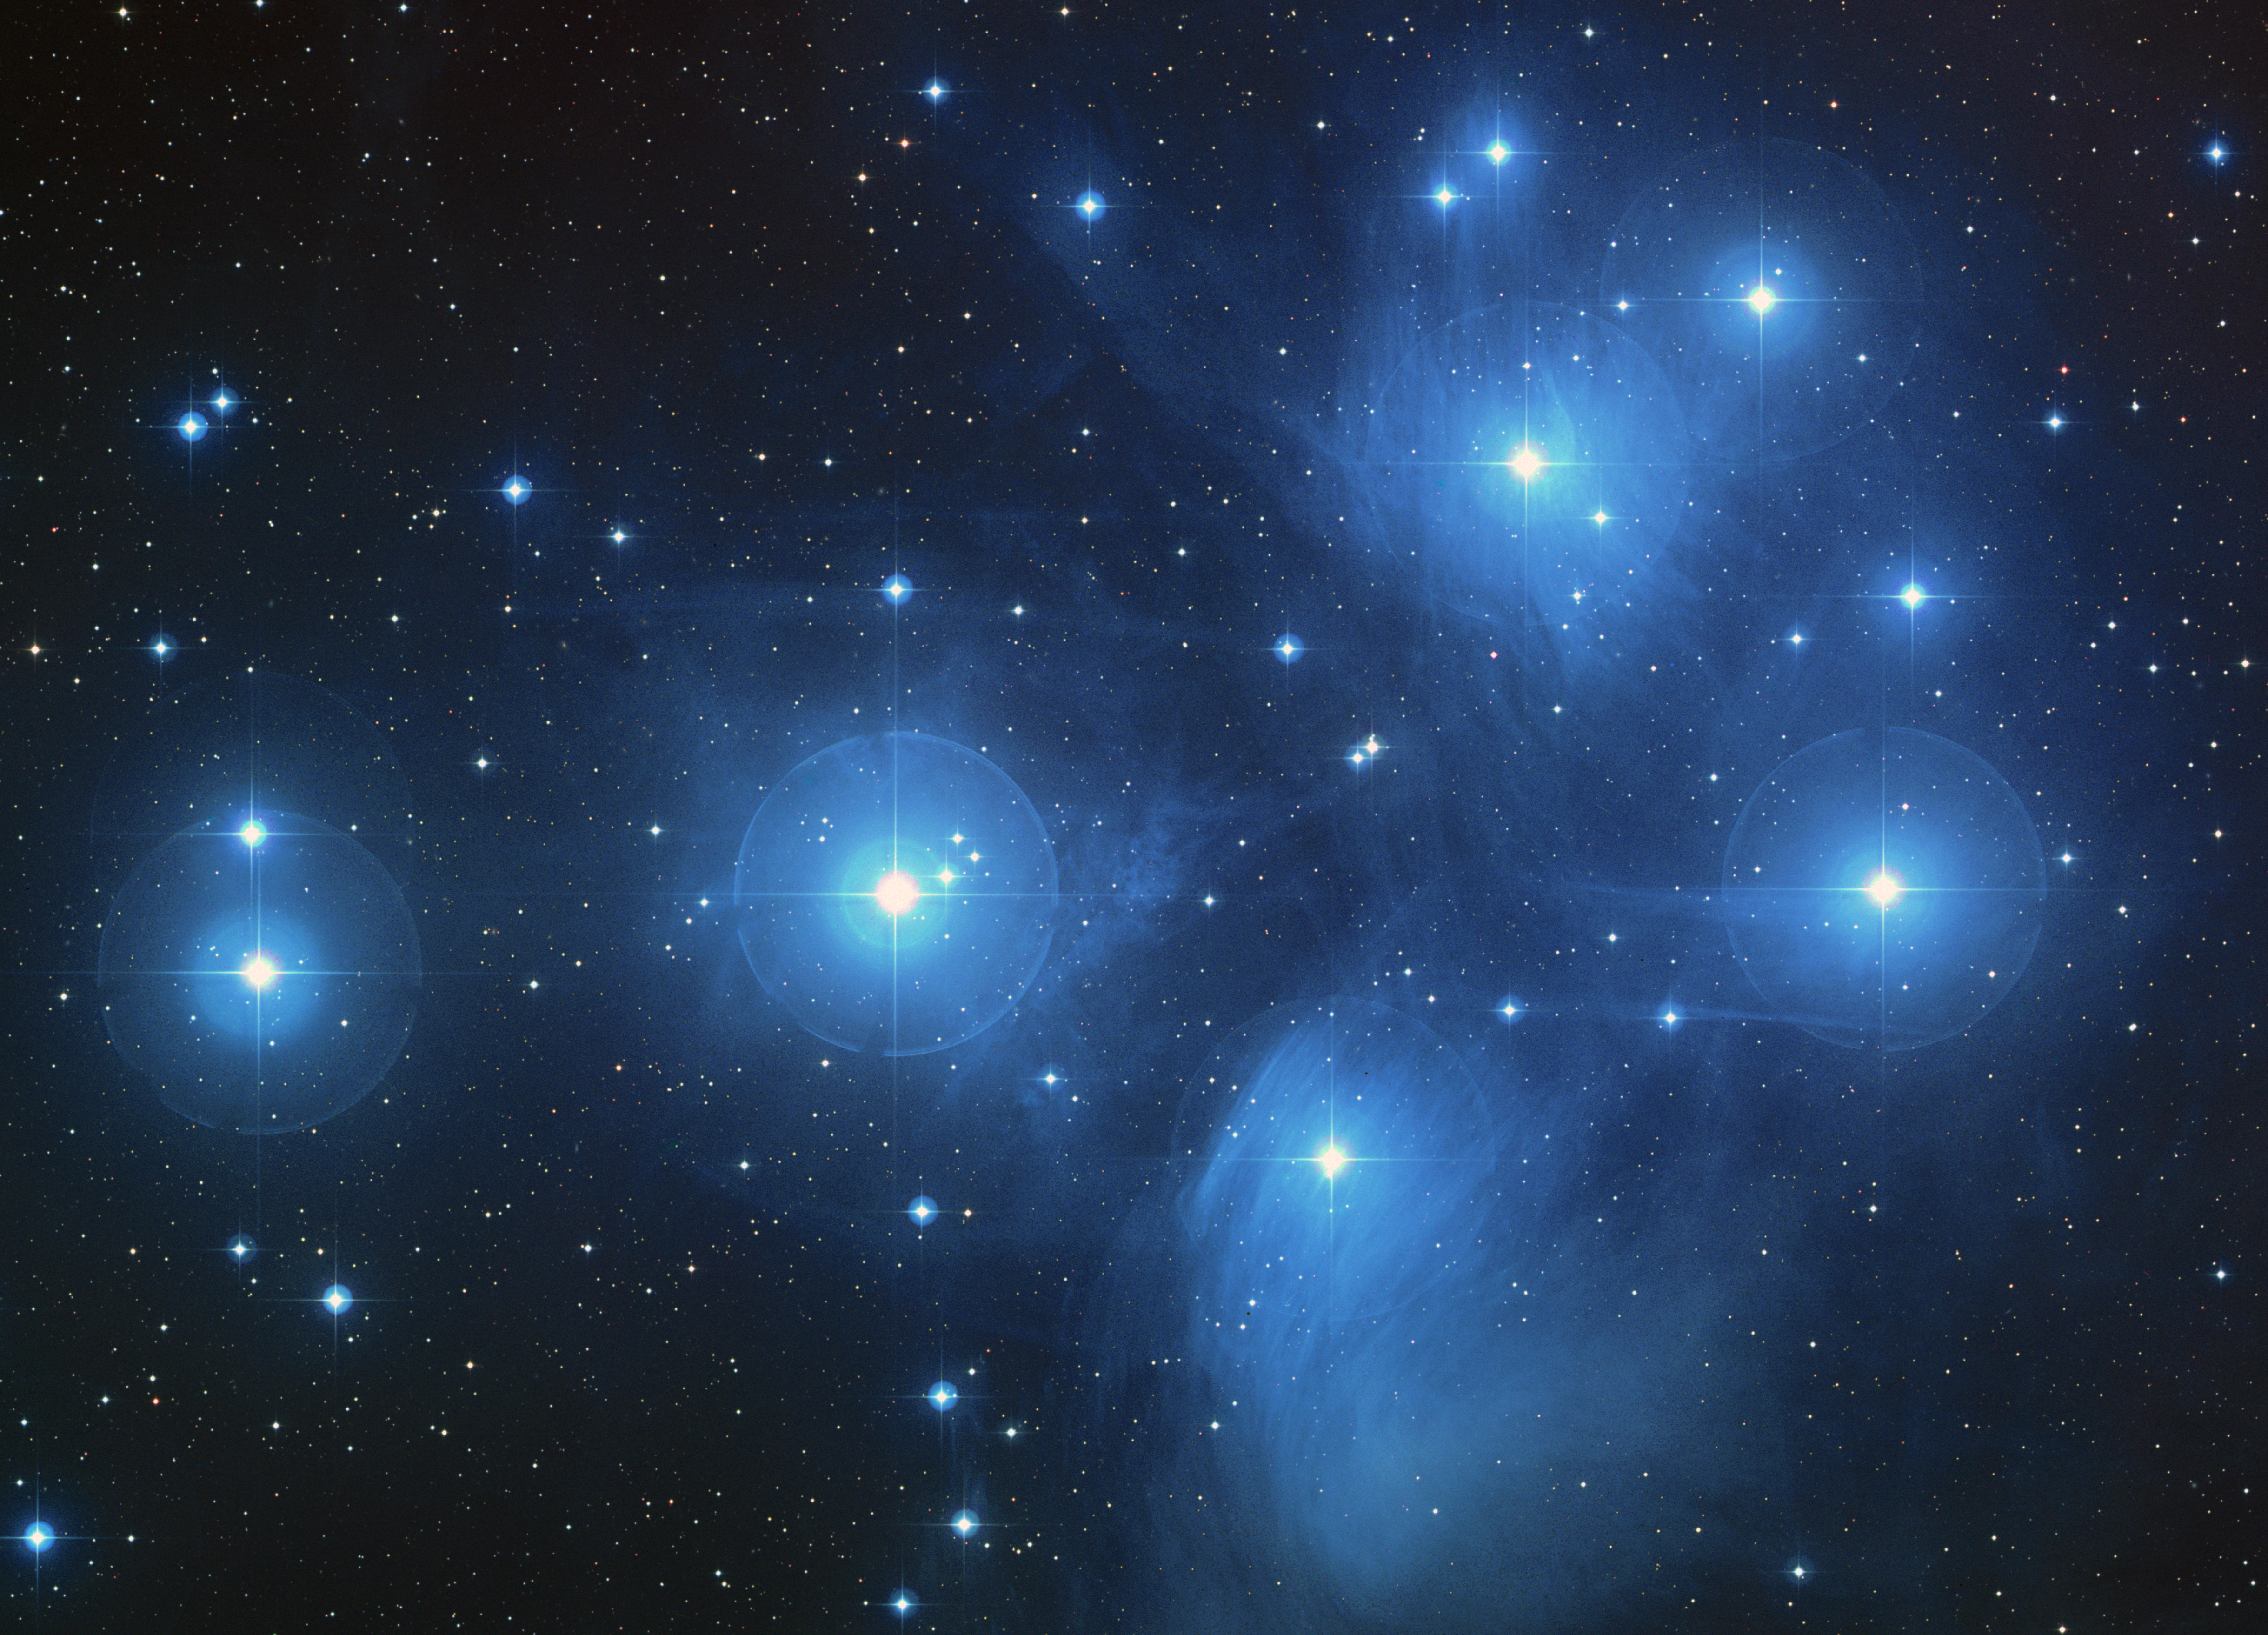
\includegraphics[width=6.6cm]{figures/Pleiades_large.jpeg}
\caption*{Credits: NASA, ESA, AURA/Caltech, Palomar Observatory,
  Public Domain,
  https://commons.wikimedia.org/w/index.php?curid=7805481}
\end{figure}
\end{minipage}
\begin{minipage}{0.5\linewidth}
\begin{figure}
\includegraphics[width=5.5cm]{figures/Ages_of_clusters_prialnik.png}
\caption*{Credits: Prialnik}
\end{figure}
\end{minipage}
\begin{itemize}
\item Main-sequence lifetimes are reflected by stellar clusters.
\end{itemize}
}
%
%
\frame{
\frametitle{Main-sequence phase}
\begin{minipage}{0.49\linewidth}
\begin{itemize}
\item Age of the cluster can be estimated from the \emph{turn-off
point} of the main-sequence.
\item The distance to the cluster can be obtained from
  \emph{main-sequence fitting}.
\item All stars in the universe with mass $M\lesssim 0.7M_\odot$ are
  still in the main sequence.
\end{itemize}
\end{minipage}
\begin{minipage}{0.5\linewidth}
\begin{figure}
\includegraphics[width=5.5cm]{figures/Ages_of_clusters_prialnik.png}
\caption*{Credits: Prialnik}
\end{figure}
\end{minipage}
}
%
%
\frame{
\frametitle{Red Giant phase}
\begin{itemize}
\item Let us consider a very simplified argument for envelope
  expansion when the core collapses.
\item Consider two mass elements $\Delta m_1$ and $\Delta m_2$ at some
  radius $r_0$ from the centre of the star. Treat $m(r_0)$ as a point
  mass.
\item Assume that the mass elements move to new positions $r_1<r_0$
  and $r_2>r_0$ and that gravitational energy is conserved.
\item The new distances are related via
  \begin{equation}
    \tilde{r}_2 = \frac{1}{(2 - \tilde{r}_1^{-1})},
  \end{equation}
  where the tildes refer to normalization by $r_0$.
\item Now a change of $r_1$ by 20\% leads to an increase of $r_2$ by
  33\% and a change of $r_1$ by 50\% leads to $r_2 \rightarrow
  \infty$ (reality more complex, \blue{why?}).
\end{itemize}
}
%
%
\frame{
\frametitle{Red Giant phase}
\begin{itemize}
\item Ultimately hydrogen is depleted in the core of the star and
  burning proceeds in the surrounding shell.
\item Due to the lack of energy sources the flux through the inert
  core approaches zero and the temperature gradient decreases.
\item As the hydrogen burning shell moves outwards, the growing core
  becomes isothermal.
\item The isothermal core has a maximum stable mass ($M_{\rm c}/M
  \approx 0.13$) above which an instability (Sch\"onberg-Chandrasekhar
  instability) sets in leading to collapse.
\end{itemize}
}
%
%
\frame{
\frametitle{Main-sequence phase}
\begin{minipage}{0.49\linewidth}
\begin{itemize}
\item An isothermal core develops for stars with $M\gtrsim 2 M_\odot$.
\item The core collapses due to the Sch\"onberg-Chandrasekhar
  instability but ultimately the temperature increses and hydrostatic
  equilibrium is restored. Core contraction continues but now in
  Kelvin-Helmholtz timescale.
\item Hydrogen burning commences in a shell surrouding the core. This
  is due to the CNO-cycle which is highly $T$-dependent.
\item At sufficiently high $T$ helium burning commences.
\item Gas cools and opacity increases in envelope: convection ensues
  (dredge-up).
\end{itemize}
\end{minipage}
\begin{minipage}{0.5\linewidth}
\begin{figure}
\includegraphics[width=7cm]{figures/M7Msun_RGB_prialnik.png}
\caption*{Evolution of a $7M_\odot$ star crossing the Hertzsprung gap
  Credits: Prialnik.}
\end{figure}
\end{minipage}
}
%
%
\frame{
\frametitle{Red Giant phase and beyond}
\begin{minipage}{0.49\linewidth}
\begin{itemize}
\item In stars with $M\lesssim 2 M_\odot$ the electron degeneracy
  pressure becomes high enough that the core can grow beyond the
  Sch\"onberg-Chandrasekhar limit.
\item Nuclear reactions and degenerate electron gas are an explosive
  combination because of the thermal instability discussed on the
  previous lecture.
\item This leads to a \emph{helium flash} where large amounts of
  helium are fused into carbon in a very short period of
  time. Enormous energy release ($10^{11}L_\odot$!) goes to bring gas
  out of degeneration and absorbed by the envelope.
\end{itemize}
\end{minipage}
\begin{minipage}{0.5\linewidth}
\begin{figure}
\includegraphics[width=7cm]{figures/Evolutionary_track_1m.png}
\caption*{By Lithopsian - Own work, CC BY-SA 4.0,
  https://commons.wikimedia.org/w/index.php?curid=48486177.}
\end{figure}
\end{minipage}
}
%
%
\frame{
\frametitle{Red Giant phase and beyond}
\begin{minipage}{0.49\linewidth}
\begin{itemize}
\item This is followed by less volatile core helium burning in the
  horizontal branch.
\item In the early asymptotic giant branch (AGB) phase the core of the
  star consists of mostly carbon and oxygen, while helium and hydrogen
  continue to be burned in separated shells.
\item At later AGB stage the star undergoes thermal pulsing that is
  related to unstable helium and hydrogen shell burning. This is
  associated with strong stellar winds and sometimes expulsion of some
  of the envelope material.
\end{itemize}
\end{minipage}
\begin{minipage}{0.5\linewidth}
\begin{figure}
\includegraphics[width=7cm]{figures/Evolutionary_track_1m.png}
\caption*{By Lithopsian - Own work, CC BY-SA 4.0,
  https://commons.wikimedia.org/w/index.php?curid=48486177.}
\end{figure}
\end{minipage}
}
%
%
\frame{
\frametitle{Post-AGB phase: superwind and planetary nebula}
\begin{itemize}
\item At the end of the AGB the outer envelope of the star cools down
  and recombination, molecule, and dust formation starts to happen.
\item The outward radiation pressure starts to become important
  especially for the dust grains (\blue{Why?}). The wind picks up and
  drives strong mass loss ($\dot{M} \sim 10^{-4}M_\odot$,
  \emph{superwind}).
\item Due to the superwind, stars from the mass range $1 M_\odot \leq
  M \lesssim 9 M_\odot$ end up with cores (that develop to white
  dwarfs) in the range $0.6M_\odot$ and $1.1M_\odot$. Most end up
  around $0.6M_\odot$ (\blue{Why?})
\item When the mass loss ends the core continues to contract and heat
  up. At sufficiently high temperature ($\sim 3\cdot 10^4$~K) the
  radiation is strong enough to ionize matter in the nearly
  spherically symmetric ejecta envelope.
\item This is then observed as a \emph{planetary nebula}.
\end{itemize}
}
%
%
\frame{
\frametitle{Post-AGB phase: superwind and planetary nebula}
\begin{minipage}{0.49\linewidth}
\begin{itemize}
\item Planetary nebula is a misnomer because originally these objects
  were thought to be forming (instead of dying) solar systems.
\item The planetary nebula phase is relatively short-lived and because
  the ejected shell expands and cools and because the nuclear
  reactions in the core ultimately cease.
\item The leftover is just the core of the star which is now a white
  dwarf.
\end{itemize}
\end{minipage}
\begin{minipage}{0.5\linewidth}
\begin{figure}
\includegraphics[width=6cm]{figures/NGC7293\_2004.jpeg}
\caption*{Helix Nebula NGC7293 (Credit: Public Domain,
  https://commons.wikimedia.org/w/index.php?curid=1721117).}
\end{figure}
\end{minipage}
}
%
%
%
\end{document}
% 

